\documentclass{article}
\usepackage[margin=1in]{geometry}
\usepackage{graphicx}
\usepackage{hyperref}
 
\date{\today}
\author{Samuel Wehunt, Luke Lambert}
\title{A Deep-Q-Learner to Play Super Smash Brothers}

\begin{document}
\maketitle


In this paper, we describe the process we went through to teach an AI in the video game, Super Smash Bros. Melee, how to avoid damage by shielding, one of the available moves within the game. By using a deep reinforcement learning process, we were able to train and reward our AI in such a way that encourages shielding, while discouraging both excessive shielding and taking damage.  
\section{Introduction}
The video game, Super Smash Bros. Melee, contains so many combinations of characters, stages, items, and moves, that our initial 
approach of attempting to teach an AI to learn how to play the game in general, from this bulk of information, had to be vastly 
limited in scope. Thus, we fine-tuned our approach to focus on a single character, Fox, a single stage, Final Destination (a flat, 
easy to navigate stage), and a single move, shield. Additionally, our AI focuses exclusively on minimizing the amount of damage it 
takes, rather than attempting to maximize damage done to its opponent. As proposed in \cite{atari}, we use a Deep Q Network (DQN) in order to 
train our AI. In a typical Q-Learning algorithm, a function called a Q-function, Q\(s,a\), is used to calculate the expected future reward 
from state s and action a. Similarly, a DQN uses a neural network in order to approximate rewards, based on previous states, actions, and rewards.

To begin the process, we have a manually controlled character randomly shoot a projectile towards our AI. At each frame of gameplay, we obtain 
the game’s state, action, reward, and next state, append this to a list representing the DQN’s memory, and then train the AI with this list to 
produce a new action. In this context, a state is a representation of the AI’s x/y coordinates on the current state, as well as the x/y 
coordinates of projectiles close to the AI. The action retrieved in this context will be representative of whether the AI’s previous action was 
to either shield or to take no action. The AI receives a specific reward based on a few criterium. A reward is first given based on how much 
damage the AI has taken since the previous state; if it has taken damage, points will be deducted, while taking no damage results in no point 
deduction. Afterwards, points are rewarded for every projectile that the AI successfully blocked. In Super Smash Bros. Melee, using the shield 
for too long results in it breaking, leaving the character stunned for a number of seconds. To counter this, we deducted a small amount of points 
to our AI’s reward if both its previous and current move was to shield. Overall, this tactic results in an AI that will, over time, learn to successfully 
shield most projectiles, without overusing its shield.
\section{Background}
To accomplish these tasks, we chose to use Dolphin, a GameCube and Wii emulator with high compatibility across the majority of titles 
for both platforms. To interface with Dolphin, we used a Python 3 library called libmelee; this allowed us to interact with the game 
via controller mapping, as well as to obtain information about the game’s current state through Dolphin. To perform our deep reinforcement 
learning, we chose to use Karas, a high\-level Python neural networks deep learning library, capable of running on top of TensorFlow, CNTK, or Theano.
\section{Related Work}
After reviewing the paper, “Playing Atari with Deep Reinforcement Learning”, our project shifted focus from solely using reinforcement learning 
techniques, to adopting the authors’ proposed algorithm, the Deep Q Network \cite{atari}. As evident in the paper, the authors’ DQN technique surpassed 
previous reinforcement learning methods within the same domain on six out of the seven Atari 2600 games. This led us to believe that, although 
our domain is more complicated than the one presented in the paper, we could benefit greatly from replacing traditional Q Learning with Deep Q Learning. 
Luckily, rather than reading in the environment via raw pixel inputs, the libmelee library allowed us to interface directly with the Dolphin emulator 
in order to obtain important information about the game’s state, such as button presses and player/projectile positions.

\section{Experiments and results}
\begin{figure}[ht]
    \centering
    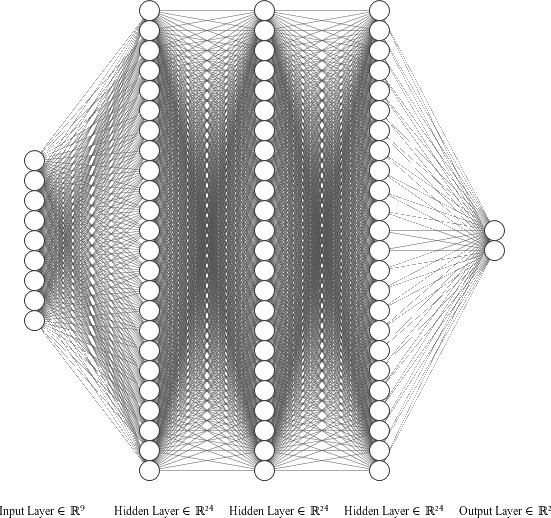
\includegraphics[width=\textwidth]{nn}
    \caption{Neural Network Architecture}
    \label{fig:nn}
\end{figure}
This project implements a deep q-learner using python and Keras, which is a framework which provides an interface
into the tensorflow library. The specific implementation and experiments are detailed below.
\subsection{Implementation}
The deep q-learner is made from a neural network consisting of 5 layers (See figure \ref{fig:nn}). The input layer consists of 9 nodes corresponding to the following input values:
\begin{itemize}
\item closest projectile x cooridnate
\item closest projectile y coordinate
\item closest projectile x velocity
\item closest projectile y velocity
\item closest projectile owner
\item closest projectile subtype
\item ai x coordinate
\item ai y coordinate
\item ai `action' (animation state)
\end{itemize}

the next three layers are densely connected hidden layers composed of 24 nodes each, and the final output layer is made up of
two nodes which maps the neural network's output to the decision of whether to shield or not to shield for that frame. Each node
in the network uses the ReLU activation function.

The experiment made use of a replay buffer in oreder to provide a long term memory to the learner, and this buffer was used periodically
to retrain on random batches of past samples so that the learner can learn from the present scenario while not forget past scenarios.

The full code and data for this project can be found at the github repository located at \url{https://github.com/Samboy218/meleeAI}

\subsection{Results}
\begin{figure}[ht]
    \centering
    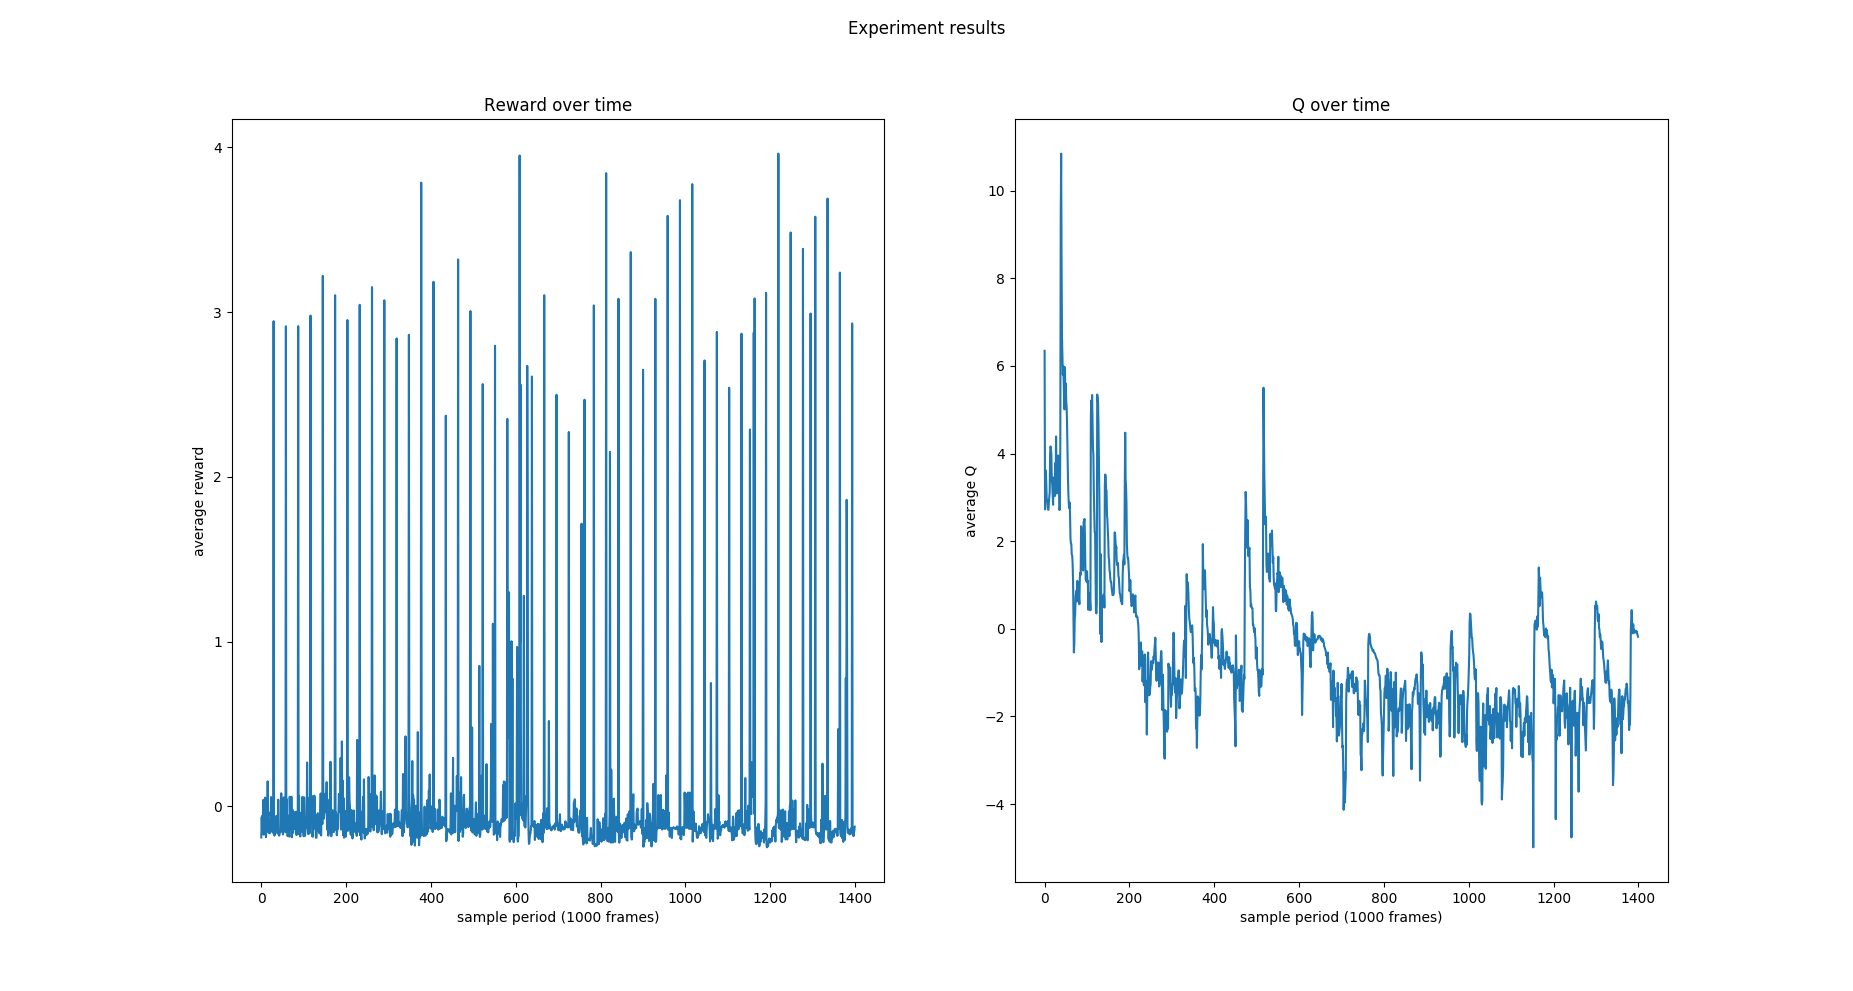
\includegraphics[width=\textwidth]{experiment}
    \caption{Experiment results}
    \label{fig:experiment}
\end{figure}
The experiment for this project was run for several hours, and during this time each frame was polled for the reward during that frame as 
well as the expected Q value for that state. These values allow one to see the general progress of the learner as it learns to perform in the
environment. Figure \ref{fig:experiment} shows the average reward and the average Q values over the experiment period. These values are 
averaged over every 1000 frames because the memory replay minibatch process was performed every 1000 frames.

The graph of the average reward is very noisy, and while there may be some general trend among the data, it is overall not useful for evaluation
of the learner, as small changes in the neural network can lead to very different actions. This phenomenon is widely documented in other literature
relating to deep Q-Learners \cite{atari}. A better metric for evaluating the learner's progress is the average Q value of predictions made by the learner.
The Q value represents the learner's expected value from taking an action, and as this increases there is an indication that the learner is 
expecting better rewards for its actions. Unfortunately, the results indicate that over time the learner performed worse at the task given to it.
While there was some improvement around the 500 time period, that improvement quickly diminished. There are several reasons this may have
happened, but the most likely culprit was the lack of data provided to the learner. The usage of the libmelee library was instrumental to this
project; however, the development of that library is limited and focused on tasks which are different from the task that this learner was given.
This means that some data which could be relevant for the learner, such as the amount of shield remaining, was unavailable for the learner to take
advantage of. Future work would involve mitigating these shortcomings by enhancing the feature set that the learner is able to take advantage of.

\begin{thebibliography}{5}
\bibitem{atari}
V. Mnih, K. Kavukcuoglu, D. Silver, A. Graves, I. Antonoglou, D. Wierstra, and M. Riedmiller, “Playing Atari with Deep Reinforcement Learning,” \textit{DeepMind Technologies}.

\bibitem{dolphin}
https://dolphin-emu.org/docs/faq/

\bibitem{keras}
https://keras.io/

\bibitem{libmelee}
https://github.com/altf4/libmelee/tree/master/melee

\end{thebibliography}
\end{document}
